In this section, we describe our proof-of-concept implementation of the system proposed in Section IV. The overall architecture is depicted in Figure \ref{fig:impel}. 

\begin{figure}[H]
  \centering
  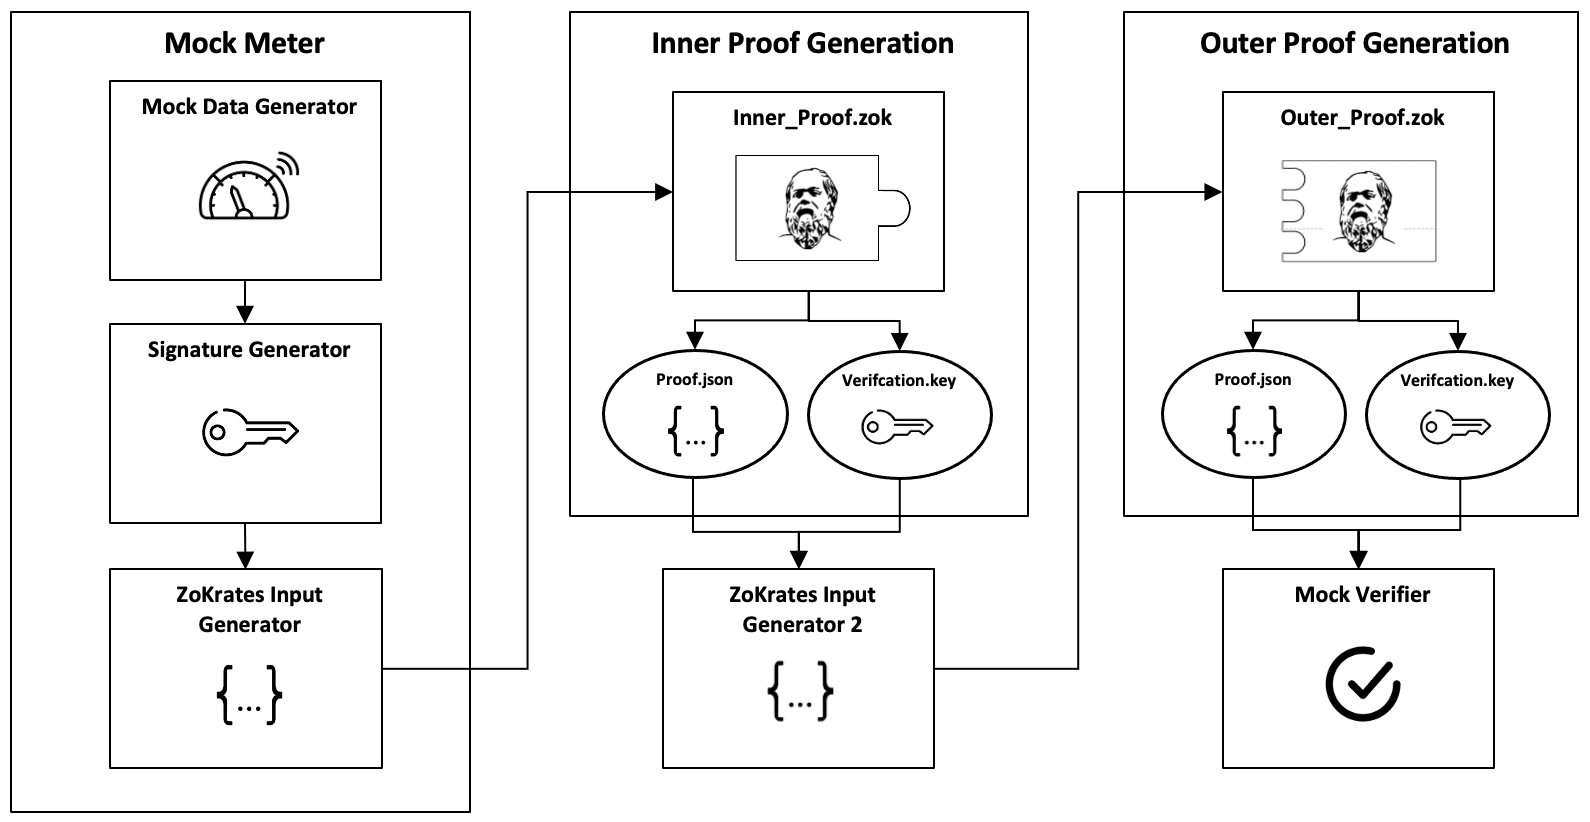
\includegraphics[width=7cm]{img/impel.png}
  \caption{Schematic illustration of the implementation's components and their interactions}
  \label{fig:impel}
\end{figure}

\subsection{Mock Meter}
Inspired by Eberthardt's et al. \cite{DecentralizedEnergyTradingMockSensor} "mock sensor for decentralized energy trading", a mock smart meter has been implemented in Python that provides energy data and generates the required input file that is utilised in the inner proof's generation. The implementation produces mocked energy data based on Gaussian regression to simulate energy data measured in kWh. Furthermore, a household internal netting or energy balance for a given interval is calculated, in order to minimise the number of variables that need to be aggregated later. 

A peculiarity is, that a specific signature is required that is compatible with the elliptic curve used in the inner proof's computation. Therefore a special implementation of the ZoKrates PyCrypto package \cite{BachelorThesisGitHub} is utilised to sign the energy readings on the decaf377 curve. 

Finally, an \texttt{inputs.json} file is created that contains all data in the correct input format for ZoKrates. 

\subsection{Inner Proof Generation}
The inner proof of integrity is computed using the mock meter's input  file. The smart meter's signature is verified and the correctness of the publicly provided net result ensured. ZoKrates' standard library does not support the for nesting required BLS12\_377 (decaf377) curve for signature verification. 
Therefore, Mehrpoya's implementation of the decaf377 curve in ZoKrates \cite{BachelorThesisGitHub} is utilised and the corresponding \texttt{verifyEddsa} function imported that allows the verification of the smart meter's signature inside the inner proof.

\subsection{ZoKrates Input Generator 2}
The input generator collects all \texttt{proof.json} files and \texttt{verification.key} files from all households and streamlines them into a suitable json format that can be utilised to compute the outer proof. 

\subsection{Outer Proof Generation}
The outer proof verifies the correctness of all inner proofs as well as the compliance of the aggregated energy balances with the threshold. As the outer proof utilises a different elliptic curve than the inner proof, negative energy balances are converted from Bls3\_77 to bw6\_761.

\subsection{Mock Verifier}

Since the nested proof compiled on the bw6\_761 curve is not verifiable on Ethereum today, a mock verifier in Python is also implemented, that verifies the proof inside a ZoKrates environment. 